\documentclass[noback]{poster}

%%\documentclass[noback,portrait]{poster}
%% To make a poster in portrait, use the "portrait" option to
%% documentclass as shown above.

\usepackage{mathptmx}
\usepackage{xspace}
\usepackage{amsmath}
\usepackage{pifont}
\usepackage{psfrag}

\usepackage{wrapfig}


\begin{document}

%% Not needed for most posters.
%%\renewcommand{\poster@ancimage}{/tmp/empty.ps}
\newcommand{\don}{\ensuremath{d_{\textsc{ON}}}}
\newcommand{\doff}{\ensuremath{d_{\textsc{OFF}}}}
\newcommand{\dsoma}{\ensuremath{d_{\textsc{SOMA}}} \xspace}
\newcommand{\um}{\ensuremath{\mu \text{m}}\xspace}
\newcommand{\dmin}{d$_{\textup{min}}$\xspace}

\title{Joshua: An Open Source Toolkit for Parsing-based Machine Translation}
%%\subtitle{The poster subtitle here}
\author{Zhifei Li,
Chris Callison-Burch,
Chris Dyer,$^\dagger$
Juri Ganitkevitch,$^+$
Sanjeev Khudanpur, 
Lane Schwartz,$^\star$
Wren N.G. Thornton,
Jonathan Weese,
{\textnormal{and}} Omar F. Zaidan}
\address{Johns Hopkins University,
$^\dagger$University of Maryland,
$^+$RWTH Aachen University,
$^\star$University of Minnesota }

\makeposter

\section{Introduction}


Beta retinal ganglion cells (RGCs) are labelled ON-centre or
OFF-centre, depending on their response to light (Fig.~1). Cell bodies
of each type form a semi-regular pattern, termed ``retinal mosaics''.
We do not yet know how the mosaics of ON- and OFF-centre cells emerge
during development:
\begin{itemize}
\item A population of undifferentiated beta cells may divide into two
  types during development through heterotypic interactions, possibly
  mediated by activity.
\item The two types of cell may develop independently of each other.
\end{itemize}

Previous statistical approaches are based on testing for
\textit{statistical independence} between ON and OFF cells. This is
not scientifically relevant when both types of neuron are located in
the same layer, since the constraint that two neurons cannot then
occupy the same (x,y)-location rules out independence \textit{a
  priori}.

\centerline{\includegraphics[width=18cm]{figs/rachel_dendrites1a.ps}
  \begin{pspicture}(0,0)(0,0)
    %%\showgrid
    \rput[l](-2,1){\small OFF}
    \rput[l](-5,1){\small ON}
    \rput[lb](-5.5,4.7){\small mature}
    \rput[lb](-16,4.7){\small immature}
    \rput[lb](-9.2,1){\small IPL}
  \end{pspicture}
}

\textbf{Figure 1}: \textit{Development of stratification in beta RGCs
  (drawing from Wong \& Ghosh, 2002).  Stratification reflects
  functional class.}

\paragraph{\blue Approach:} we fit models of the joint spatial pattern
which respect the constraint that no two neurons can be separated by
less than their soma diameter.  If model replicates real maps without
requiring heterotypic interactions, this might suggest heterotypic
interactions do not occur during development.

\centerline{
  \includegraphics[angle=-90,width=23cm]
  {figs/w81s_sim_map.ps}}

\vspace*{4mm}
\centerline{\textbf{Figure 2}: \textit{Real (W81s; W\"{a}ssle et al., 1981)
  and simulated RGC mosaics.}}

\section{Methods}


\begin{itemize}
\item \dmin model (Galli-Resta et al., 1997) adapted to bivariate case
  (Fig.~3).  Size of homotypic exclusion zones drawn from a Normal
  distribution (mean $\pm$ s.d.); heterotypic exclusion zone fixed at
  soma diameter.
  
\item Model parameters varied to find best fit to real maps (M623 and
  W81s) for:
  \begin{enumerate}
  \item $L(t)$ --- mean (scaled) number of cells within distance
    $t$ of a cell. L functions are cumulative versions of DRP
    (Rodieck, 1991).
  \item regularity index --- mean/s.d. of the distance to
    nearest-neighbour.
    
  \item  fraction of $1^{st}$, $2^{nd}$, $3^{rd}$, or all,
    nearest neighbours of opposite type.
  \end{enumerate}
\end{itemize}  
\columnbreak

{
\centerline{\includegraphics[angle=-90,width=28cm]
  {figs/show_birthdeath.ps}}
}

\vspace*{5mm} \textbf{Figure 3}: \textit{Bivariate \dmin model. On and
  off-centre cells are initially located randomly throughout the
  array.  All cells are then moved within the array according to the
  following procedure.  A cell is selected (1) and repositioned
  randomly (e.g.  at 4) avoiding homotypic exclusion zones (dotted
  circles; 2) and smaller heterotypic zones (solid red circles, which
  are cell bodies of opposite type; 3).  One sweep consists of moving
  all cells in the array once.  Cells are moved for many sweeps to
  allow the patterns to stabilise.}

\vspace*{-10mm} 
\section{Results}


\begin{pspicture}(0,0)(0,0)
  \rput(27,2){{\includegraphics[width=13cm]{figs/w81on_drp.ps}}}
  \rput(24,-0.5){\psline[arrows=<->,arrowsize=10pt,arrowinset=0](-2,-2)}
\end{pspicture}
\begin{minipage}[r]{19cm}
  Both fields could be replicated by bivariate \dmin model (Table 1;
  Fig.~2, 4, 5).  DRP to right shows equivalent DRP for an L function.
\vspace*{5mm}
\end{minipage}


\centerline{\includegraphics[width=\linewidth]{figs/m623_4poster.ps}}

\textbf{Figure 4}: \textit{Results for field M623.  Red lines indicate
experimental data; black lines indicate envelope from 99 simulations.
Dashed blue lines indicate the expectation of L for a Poisson pattern.
In strip charts, each black dot indicates one simulation, and dotted
black line indicates median.}

\columnbreak


\centerline{\includegraphics[width=\linewidth]{figs/w81s_4poster.ps}}
\centerline{
  \textbf{Figure 5}: \textit{Results for field W81s (same format as Fig.~4).}}


\vspace*{20mm}

%% Try to align numbers; not perfect but works.
\def\0{\hbox{\phantom{\footnotesize\rm 1}}}%.
\def\tabcolsep{4mm}
\begin{center}
  \begin{tabular}{cccccc}
    \hline
    field &    \# ON &  \# OFF & \don       & \doff       & soma \\
    %%          & (\#)  & (\#) & (\um)      &  (\um)      & (\um) \\
    \hline
    W81s  &    65 &   70 & $116 \pm 20$ \um  & $130  \pm 25$ \um & \09 \um\\
    M623  &    74 &   82 & $100 \pm 13$ \um  & $\090 \pm 15$ \um & 15 \um \\
    \hline
  \end{tabular}
\end{center}

\vspace*{5mm}

\textbf{Table~1}: \textit{Best-fit parameters of the \dmin model to the two
datasets.  \don\  and \doff: mean $\pm$ s.d. of homotypic exclusion
zones; soma: diameter of heterotypic exclusion zone.}


\vspace*{-1cm}

\section{Conclusions}

\begin{itemize}
\item Beta RGC maps can be simulated with limited interactions
  between the two mosaics.  Heterotypic interactions are limited to
  preventing somal overlap.
  
\item Confirms general principle that mosaics are \textit{functionally
    independent} of each other (Rockhill et al., 2000).
  
\item Previous model suggested fixed dependency between two mosaics
  (Zhan \& Troy, 2000); may be by-product of model implementation.

%% \item The same mechanism may account for bivariate horizontal cell mosaics.
  
\item Functional implications of independence in arrays?

\item Caveats: model works with adult maps (ignoring developmental
  processes, such as cell death).  Limited data sets (n=2).
  Interactions between dendritic refinement and soma positioning unknown.

\end{itemize}

{\blue \bfseries Acknowledgements:} Wellcome Trust (SJE) and NIH
EY06669 (JBT).  Thanks to Heinz W\"{a}ssle for providing map W81s.

\end{document}

% LocalWords:  RGCs
